\section{Ainul Filiani}
\begin{enumerate}
\item Apa itu fungsi library matplotlip ?

Data yang kita olah tentu tidak bagus apabila ditampilkan begitu saja dengan tabel hitam saja kepada investor atau manajemen. Bila ditampilkan dengan sejumlah grafik berwarna pasti akan terlihat lebih menarik ketika melihatnya. Matplotlib membantu kita untuk memvisualisasikan data dengan lebih indah dan rapi.
Ada plot untuk menampilkan data dengan cara 2D atau 3D. Sehingga kita dapat menampilkan data yang telah kita olah sesuai kebutuhan. Matplotlib pun terintegrasi dengan iPython Notebook atau Jupyter dimana kita dapat membuat sebuah buku interaktif yang dapat diberi penjelasan dan kode yang disisipkan begitupun hasil plottingnya.
Matplotlib adalah library paling banyak atau sering digunakan oleh data science untuk menyajikan datanya ke dalam visual yang lebih baik.

\item jelaskan langkah-langkah membuat sumbu X dan Y di matplotlip?

untuk membuat sumbu x dan y kita bisa menggunakan list untuk mempermudah penyimpanan nilai setiap sumbunya.
contoh pembuatannya: 
\lstinputlisting[firstline=9, lastline=10]{src/6/1174073/teori/1174073.py}

\item jelaskan bagaimana perbedaan fungsi dan cara pakai untuk berbagai jenis (bar, histogram, dll). jenis plot di matplotlip ?  

Untuk perbedaan fungsi plot yang digunakan adalah bentuk bentuk grafik yang akan di tampilkan sesuai dengan perintah yang digunakan pada pemogramannya.
Dan untuk cara pengguna plot tersebut sebagai berikut
\begin{itemize}
    \item line
    Perintah yang digunakan untuk membuat grafik line sebagai berikut.
    \lstinputlisting[firstline=12, lastline=14]{src/6/1174073/teori/1174073.py}
    \item bar
    Dalam Penggunaan plot bar koordinat x nya itu yang awal, dan untuk Y nya adalah yang kedua
    \lstinputlisting[firstline=16, lastline=25]{src/6/1174073/teori/1174073.py}
    \item histogram
    Dalam penggunaan plot histogram titik x nya bisa tidak sama dengan titik Y.
    untuk penggunaannya bisa sebagai berikut.
    \lstinputlisting[firstline=27, lastline=34]{src/6/1174073/teori/1174073.py}
    \item scatter
    Untuk penggunaa plot scatter atau bisa juga d bilang diagram titik.
    Contoh dari penggunaannya bisa dilihat sebagai berikut.
    \lstinputlisting[firstline=36, lastline=49]{src/6/1174073/teori/1174073.py}
    \item Stack plot
    Untuk penggunaan stack plot ini seperti diagram line, tapi ada fill colornya,jadi antar line itu bisa berdekatan.
    Berikut Contoh penggunaannya
    \lstinputlisting[firstline=82, lastline=92]{src/6/1174073/teori/1174073.py}
\end{itemize} 

\item Jelaskan bagaimana cara menggunakan legend dan lebel serta kaitannya dengan fungsi tersebut 

Untuk menggunakan legend dan label bisa di lihat dibawah ini
\lstinputlisting[firstline=20, lastline=22]{src/6/1174073/teori/1174073.py}
penggunaan legend itu untuk mempermudahkita dalam membaca grafik, legend itu sendiri berisi info info dari grafik yang ada seperti nama, kemudian bentuk dan warna.
kemudian untuk label itu sendiri digunakan untuk membedakan nama titik X dan titik Y.

\item Jelaskan apa fungsi dari subplot di matplotlib dan agaimana cara kerja dari fungsi subplot, sertakan ilustraasi dan gambar sendiri dan apa parameternya jika ingin menggambar plot dengan 9 subplot didalamnya ? 

fungsi dari subplot dari matplotlib untuk bisa membuat lebih dari 1 grafik dalam sebuah program.
untuk cara kerjanya sendiri bisa d cek sebagai berikut
\lstinputlisting[firstline=94, lastline=104]{src/6/1174073/teori/1174073.py}
untuk parameternya sendiri saya menggunakan x dan y x sebagai koordinat x dan y sebagai koordinat y.
\begin{figure}[H]	
    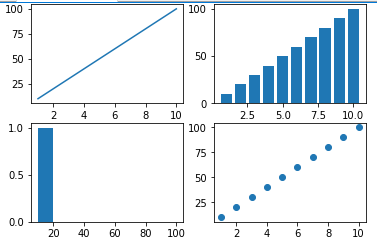
\includegraphics[width=5cm]{figures/6/1174073/teori/satu.png}
    \centering
    \caption{SubPlot}
\end{figure}

\item sebutkan semua pparameter color yang bisa digunakan contoh: m,c,r,k,...

Untuk parameter color yang bisa digunakan terdiri dari 2 type warna.

Tipe Warna RGB

Untuk keterangannya sebagai berikut
\begin{enumerate}
\item R untuk warna Red atau Merah
\item G untuk warna Green atau Hijau
\item B untuk warna Blue atau Biru
\end{enumerate}
Tipe warna CMYK

Untuk keterangannya sebagai berikut
\begin{enumerate}
\item    C untuk warna Cyan atau Biru Muda
\item    M untuk warna Mangenta atau Merah Tua
\item    Y untuk warna Yellow Atau Kuning
 \item   K untuk warna blacK atau Hitam
\end{enumerate}

\item Jelaskan bagaimana cara kerja dari fungsi hist, sertakan ilustrasi dan gambar sendiri?

Untuk fungsi histogram ini kedua titik koordinat boleh tidak sama. Misalnya x nya ada 10 nilai sedangkan Y nya ada 5 nilai, itu tidak akan jadi masalah karena diagram ini digunakan untuk mendata usia dari rentang tertentu atau kebutuhan lainnya.
Ini merupakan contoh dari penggunaan histogram
\lstinputlisting[firstline=27, lastline=34]{src/6/1174073/teori/1174073.py}
dan ini merupakan grafik histogram tersebut.
\begin{figure}[H]	
    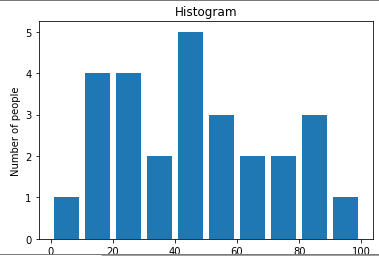
\includegraphics[width=5cm]{figures/6/1174073/teori/histogram.png}
    \centering
    \caption{Diagram Histogram}
\end{figure}

\item jelaskan lebih mendalam tentang parameter dari fungsi pie diantaranya labels, colors,startangle, shadow, explode, autopct.

Berikut penjelasan tentang parameter yang ada dalam pie chart
\begin{itemize}
    \item label
    Label digunakan untuk mempermudah pembaca dalam membaca diagram pie
    \item color
    warna digunakan untuk membedakan antar data
    \item startangle
    Digunakan untuk sudut yang digunakan untuk memulai diagram pie tersebut
    \item shadow
    bayangan digunakan untuk membuat bayangan dari setiap diagram pie yang menonjol
    \item explode
    explode digunakan untuk mengeluarkan suatu data agar data tersebut terlihat menonjol
    \item autopct
    Digunakan sesuai dengan berapa angka dibelakang koma yang kita inginkan
\end{itemize} 
\end{enumerate}
%%%%%%%%%%%%%%%%%%%%%%%%%%%%%%%%%%%%%%%%%%%%%%%%%%%%%%%%%%%%%%%
\section{Sekar Jasminei}
\begin{enumerate}

\item 1. Apa itu fungsi library Matplotlib
Matplotlib adalah sebuah library pada python yang digunakan untuk membuat diagram. Library ini biasanya menghasilkan ploting 2D.\\

Ada plot untuk menampilkan data secara 2D atau 3D. sehingga kamu dapat menampilkan data yang telah kamu olah sesuai kebutuhan. Matplotlib pun terintegrasi dengan ipython notebook atau jupyter dimana kamu dapat membuat sebuah buku interaktif yang dapat diberi penjelasan dan kode yang disisipkan begitupun hasil plottingnya.\\

\item 2. Jelaskan langkah-langkah membuat sumbu X dan Y di matplotlib.
untuk membuat sumbu x dan y kita bisa membuatnya menggunakan list untuk mempermudah penyimpanan nilai setiap sumbunya.\\
\lstinputlisting[firstline=9, lastline=11]{src/6/1174075/teori/1174075.py}

\item 3. Jelaskan bagaimana perbedaan fungsi dan cara pakai untuk berbagai jenis(bar,histogram,scatter.dll) jenis plot di matloptlib
Untuk perbedaan fungsi plot yang digunakan adalah bentuk bentuk grafik yang akan di tampilkan sesuai dengan perintah yang digunakan pada pemogramannya.\\

line itu untuk perintah yang digunakan untuk membuat grafik line sebagai berikut.\\
\lstinputlisting[firstline=12, lastline=15]{src/6/1174075/teori/1174075.py}
Bar itu di dalam Penggunaan plot bar koordinat x nya itu yang awal, dan untuk Y nya adalah yang kedua.\\
\lstinputlisting[firstline=16, lastline=26]{src/6/1174075/teori/1174075.py}
Histrogram itu di dalam penggunaan plot histogram titik x nya bisa tidak sama dengan titik Y. untuk penggunaannya bisa sebagai berikut.\\
\lstinputlisting[firstline=27, lastline=35]{src/6/1174075/teori/1174075.py}
scatter untuk penggunaa plot scatter atau bisa juga d bilang diagram titik.\\
\lstinputlisting[firstline=36, lastline=50]{src/6/1174075/teori/1174075.py}
Stack plot untuk penggunaan stack plot ini seperti diagram line, tapi ada fill colornya,jadi antar line itu bisa berdekatan.\\
\lstinputlisting[firstline=82, lastline=92]{src/6/1174075/teori/1174075.py}

\item 4. Jelaskan bagaimana cara menggunakan legend dan label serta kaitannya dengan fungsi tersebut.
Contoh source code lengkap disertai dengan link "editor" untuk mencoba (try it) dan melihat hasil (preview) kode.\\

Elemen yang akan ditambahkan ke legenda ditentukan secara otomatis, ketika Anda tidak memberikan argumen tambahan.\\

Garis-garis spesifik dapat dikecualikan dari pemilihan elemen legenda otomatis dengan mendefinisikan label dimulai dengan garis bawah.\\

\item 5. Jelaskan apa fungsi dari subplot di matplotlib dan fungsi dari subplot dari matplotlib untuk bisa membuat lebih dari 1 grafik dalam sebuah program.\\

Misalnya, kita dapat membuat sumbu inset di sudut kanan atas sumbu lain dengan mengatur posisi x dan y ke 0,65 yaitu, mulai dari 65 peren dari lebar dan 65 persen  dari ketinggian gambar dan x dan y meluas ke 0,2 yaitu, ukuran sumbu adalah 20 persen  dari lebar dan 20persen dari tinggi gambar.\\

Simple Grids of Subplots itu kebutuhan yang cukup umum sehingga Matplotlib memiliki beberapa rutinitas kenyamanan yang membuatnya mudah dibuat. Level terendah adalah plt.subplot (), yang membuat subplot tunggal di dalam kisi. Seperti yang Anda lihat, perintah ini membutuhkan tiga argumen bilangan bulat — jumlah baris, jumlah kolom, dan indeks plot yang akan dibuat dalam skema ini, yang berjalan dari kiri atas ke kanan bawah.\\

The Whole Grid in One Go itu  membuat grid besar subplot, terutama jika Anda ingin menyembunyikan label sumbu x dan y pada plot bagian dalam. Untuk tujuan ini, plt.subplots () adalah alat yang lebih mudah digunakan.\\
\lstinputlisting[firstline=94, lastline=104]{src/6/1174075/teori/1174075.py}
 
\item 6. Sebutkan semua parameter color yang bisa digunakan(contoh: m,c,r,k,...dkk)
Tipe Warna RGB
    Untuk keterangannya sebagai berikut
    R untuk warna Red atau Merah
    G untuk warna Green atau Hijau
    B untuk warna Blue atau Biru.\\
    
Tipe warna CMYK
    Untuk keterangannya sebagai berikut
    C untuk warna Cyan atau Biru Muda
    M untuk warna Mangenta atau Merah Tua
    Y untuk warna Yellow Atau Kuning
    K untuk warna blacK atau Hitam.\\

\item 7. Jelaskan bagaimana cara kerja dari fungsi hist , sertakan ilustrasi dan gambar sendiri.
Untuk fungsi histogram ini kedua titik koordinat boleh tidak sama. Misalnya x nya ada 10 nilai sedangkan Y nya ada 5 nilai, itu tidak akan jadi masalah karena diagram ini digunakan untuk mendata usia dari rentang tertentu atau kebutuhan lainnya.\\

Ini merupakan contoh dari penggunaan histogram.\\

\item 8. Jelaskan lebih dalam tentang parameter dari fungsi pie diantaranya labels , color , startangle , shadow , explode , autopct.
Jika jumlah x <1, maka nilai x memberikan area fraksional secara langsung dan array tidak akan dinormalisasi.\\

labels : Label digunakan untuk mempermudah pembaca dalam membaca diagram pie.\\

color : warna digunakan untuk membedakan antar data.\\

startangle : Digunakan untuk sudut yang digunakan untuk memulai diagram pie tersebut.\\

shadow :  bayangan digunakan untuk membuat bayangan dari setiap diagram pie yang menonjol.\\

explode : explode digunakan untuk mengeluarkan suatu data agar data tersebut terlihat menonjol.\\

autopct : Digunakan sesuai dengan berapa angka dibelakang koma yang kita inginkan.\\
\end{enumerate}
%%%%%%%%%%%%%%%%%%%%%%%%%%%%%%%%%%%%%%%%%%%%%%%%%%%%%%%%%%%%%%%%%%%%%%%%%%%%%%%%%%%%%%%%%%%%%%%%%%%

\section{Kaka Kamaludin}
\subsection{Soal 1}
Matplotlib merupakan library python yang berfungsi untuk mengasilkan plot yang di paparkan dengan toolkit GUI yang interaktif.

\subsection{Soal 2}
penulisan Sumbu x dan Y, pada plt.plot(xxx, yyy) diwali dengan sumbu x lalu y.
\lstinputlisting[firstline=1, lastline=13]{src/6/1174067/Teori/1174067_teori.py}


\subsection{Soal 3}
\begin{itemize}
	\item Line Plot, berfungsi untuk menamplikan data yang berkelanjutan dalam priode tertentu.
	\lstinputlisting[firstline=15, lastline=18]{src/6/1174067/Teori/1174067_teori.py}
	
	\item Pie Chart, berfungsi untuk menamplikan bagian suatu data terhadap jumlah keseluruhan secara proporsional. 	setiap bagian data dihitung dalam persentase. pie chart berbentuk bulat seperti potongan kue.
	\lstinputlisting[firstline=20, lastline=42]{src/6/1174067/Teori/1174067_teori.py}
	
	\item Bar Chart, berfungsi sebagai perbandingan beberapa kategori data, ditampilkan dalam bentuk batang.
	\lstinputlisting[firstline=43, lastline=53]{src/6/1174067/Teori/1174067_teori.py}
	
	\item Scatter Chart, biasa digunakan untuk pengujian pola hubungan antara dua variable.
	\lstinputlisting[firstline=54, lastline=69]{src/6/1174067/Teori/1174067_teori.py}
	
	\item Histogram Chart, berfungsi untuk perbandingan data dalam bentuk range.
	\lstinputlisting[firstline=70, lastline=79]{src/6/1174067/Teori/1174067_teori.py}
	
	\item Stack Chart,.
	\lstinputlisting[firstline=80, lastline=101]{src/6/1174067/Teori/1174067_teori.py}		
\end{itemize}

\subsection{Soal 4}
Legend dan Label berfungsi untuk mempermudah dalam pembacaan chart tersebut. contohnya:
\lstinputlisting[firstline=102, lastline=119]{src/6/1174067/Teori/1174067_teori.py}

\subsection{Soal 5}
sublpot berfungsi untuk membuat plot lebih dari 1, contoh:
\lstinputlisting[firstline=120, lastline=148]{src/6/1174067/Teori/1174067_teori.py}

\subsection{Soal 6}
parameter color bisa dibuat dengan menggunakan float value(0.1, 0.2, 0.5, 0.3), hex ('\# 0F0F0F' atau '\#0F0F0F0F'), xkcd color ('xkcd:sky blue'), Tableau Colors ('tab:gray')
\begin{itemize}
    \item Tipe Warna RGB

    R untuk warna Red atau Merah,
    G untuk warna Green atau Hijau,
    B untuk warna Blue atau Biru,
    \item Tipe warna CMYK

    C untuk warna Cyan atau Biru Muda,
    M untuk warna Mangenta atau Merah Tua,
    Y untuk warna Yellow Atau Kuning,
    K untuk warna black atau Hitam
\end{itemize}
\lstinputlisting[firstline=149, lastline=169]{src/6/1174067/Teori/1174067_teori.py}

\subsection{Soal 7}
Untuk fungsi histogram ini kedua titik koordinat boleh tidak sama. Misalnya x nya ada 10 nilai sedangkan Y nya ada 5 nilai, itu tidak akan jadi masalah karena diagram ini digunakan untuk mendata usia dari rentang tertentu atau kebutuhan lainnya.
	\lstinputlisting[firstline=170, lastline=177]{src/6/1174067/Teori/1174067_teori.py}

\subsection{Soal 8}
\begin{itemize}
    \item label
    Label digunakan untuk mempermudah pembaca dalam membaca diagram pie
    \item color
    warna digunakan untuk membedakan antar data
    \item startangle
    Digunakan untuk sudut yang digunakan untuk memulai diagram pie tersebut
    \item shadow
    bayangan digunakan untuk membuat bayangan dari setiap diagram pie yang menonjol
    \item explode
    explode digunakan untuk mengeluarkan suatu data agar data tersebut terlihat menonjol
    \item autopct
    Digunakan sesuai dengan berapa angka dibelakang koma yang kita inginkan
\end{itemize}

%%%%%%%%%%%%%%%%%%%%%%%%%%%%%%%%%%%%%%%%%%%%%%%%%%%%%%%%%%%%%%%%%%%%%%%%%%%%%%%%%%%%%%%%%%%%%%%%%%%
\section{Alvan Alvanzah/1174077}
\subsection{Pemahaman Teori}

\begin{enumerate}
    \item Apa itu fungsi library matplotlib
    \par Matplotlib berfungsi untuk memvisualkan data dengan lebih indah dan rapi dengan menampilkan data secara 2D. Matplotlib mencoba membuat hal-hal mudah menjadi mudah dan hal-hal sulit menjadi mungkin. Dengan Matplotlib dapat membuat plot, histograms, power spectra, bar charts, errorcharts, scatterplots, dll.
    
    \item Jelaskan langkah-langkah membuat sumbu X dan Y di matplotlib.
    \begin{itemize}
        \item pertama import library matplotlib.
        \item kedua membuat isi dari variabel sumbu x dan y.
        \item ketiga tampilkan hasil dari sumbu x dan y.
    \end{itemize}
    \lstinputlisting[firstline=8, lastline=13]{src/6/1174077/teori/1174077.py}
    
    \item Jelaskan bagaimana perbedaan fungsi dan cara pakai untuk berbagai jenis (bar, histogram, scatter, line, dll) jenis plot di matplotlib.
    \par Untuk perbedaan fungsi plot yang digunakan adalah bentuk-bentuk grafik yang akan di tampilkan sesuai dengan perintah yang digunakan pada pemogramannya.
    Dan untuk cara pengguna plot tersebut sebagai berikut:
    \begin{itemize}
        \item bar
        
        Dalam Penggunaan plot bar koordinat x nya itu yang awal, dan untuk Y nya adalah yang kedua.
        \lstinputlisting[firstline=15, lastline=25]{src/6/1174077/teori/1174077.py}
        \item histogram
        
        Dalam penggunaan plot histogram titik x nya bisa tidak sama dengan titik Y.
        \lstinputlisting[firstline=28, lastline=36]{src/6/1174077/teori/1174077.py}
        \item scatter
        
        Untuk penggunaa plot scatter atau bisa juga d bilang diagram titik.
        \lstinputlisting[firstline=39, lastline=53]{src/6/1174077/teori/1174077.py}
        \item line
        
        Perintah yang digunakan untuk membuat grafik line sebagai berikut.
        \lstinputlisting[firstline=56, lastline=59]{src/6/1174077/teori/1174077.py}
    \end{itemize}
    
    \item Jelaskan bagaimana cara menggunakan legend dan label serta kaitannya dengan fungsi tersebut.
    \begin{itemize}
        \item Untuk membuat legenda pada plot dapat menggunakan syntax fungsi legend pada MATLAB.
        \lstinputlisting[firstline=21, lastline=21]{src/6/1174077/teori/1174077.py}
        \item Untuk menambah label pada garis sumbu pada grafik dapat menggunakan syntax fungsi xlabel dan fungsi ylabel pada MATLAB.
        \lstinputlisting[firstline=22, lastline=23]{src/6/1174077/teori/1174077.py}
        \par Kaitannya untuk memperjelas informasi dari grafik yang dibuat.
    \end{itemize}
    
    \item Jelaskan apa fungsi dari subplot di matplotlib, dan bagaimana cara kerja dari fungsi subplot, sertakan ilustrasi dan gambar sendiri dan apa parameternya jika ingin menggambar plot dengan 9 subplot di dalamnya.
    \par fungsi dari subplot dari matplotlib untuk bisa membuat lebih dari 1 grafik dalam sebuah program.
    \par untuk cara kerjanya sendiri bisa di cek sebagai berikut:
    \lstinputlisting[firstline=62, lastline=84]{src/6/1174077/teori/1174077.py}
    \par Cara penggunaannya sebagai contoh saya ambil plt.subplot(221), pada angka 2 yang pertama adalah pembagian keatas kalo kita mau bagi 3 keatas kita isi angka pertama dengan 3, angka 2 yang kedua adalah pembagian kesamping penggunaannya sama kaya angka pertama kalo kita mau ngebagi kesamping 4 kita isi angka kedua 4, dan angka 1 pada angka ketiga itu tempat disimpannya grafik yang akan dimunculkan
    
    \item Sebutkan semua parameter color yang bisa digunakan (contoh:  m,c,r,k,...  dkk)
    Parameter warna yang bisa digunakan dibagi menjadi 2 tipe:
    \begin{itemize}
	    \item RGB
	
	Untuk keterangannya sebagai berikut
    R untuk warna Red atau Merah
    G untuk warna Green atau Hijau
    B untuk warna Blue atau Biru
    
        \item CMYK
    
    Untuk keterangannya sebagai berikut
    C untuk warna Cyan atau Biru Muda
    M untuk warna Mangenta atau Merah Tua
    Y untuk warna Yellow Atau Kuning
    K untuk warna Black atau Hitam
    \end{itemize}
    
    \item Jelaskan bagaimana cara kerja dari fungsi hist, sertakan ilustrasi dan gambar sendiri.
    \par Untuk histogram kita tidak boleh memiliki isi variable x dan y yang sama. Misal x-nya ada 10 nilai sedangkan Y-nya ada 5 nilai, data tersebut tidak menjadi masalah karena pada histogram data yang dimunculkan adalah data rentang dari data variable y. Dan ini adalah contoh dari penggunaan histogram.
    \lstinputlisting[firstline=87, lastline=93]{src/6/1174077/teori/1174077.py}
    
    \item Jelaskan lebih mendalam tentang parameter dari fungsi pie diantaranya labels,colors, startangle, shadow, explode, autopct.
    \begin{itemize}
        \item Label
    
    Label digunakan untuk mempermudah pembaca yaitu memberikan nama pada variable di grafik.
    
        \item Color
    
    Warna yang dimunculkan pada setiap data.
    
        \item Startangle
    
    Startangle digunakan untuk sudut awal pada diagram pie tersebut.
    
        \item Shadow
    
    Shadow(Bayangan) digunakan untuk membuat bayangan pada setiap diagram pie yang menonjol.
    
        \item Explode

    Explode digunakan untuk mengeluarkan suatu data agar data tersebut menjadi terlihat lebih menonjol.
    
        \item Autopct
    
    Autopct digunakan menyesuaikan berapa angka yang ada dibelakang koma.
\end{itemize}
\end{enumerate}
%%%%%%%%%%%%%%%%%%%%%%%%%%%%%%%%%%%%%%%%%%%%%%%%%%%%%%%%%%%%%%%%%%%%%%%%%%%%%%%%%%%%%%%%%%%%%%%%%%%
\section{Fernando L Sihite /1174072}
	\subsection{Soal 1} 
		\begin{itemize}
			\item Apa itu fungsi library matplotlib 

			\item Matplotlib merupakan bagian dari library pada python yang biasanya digunakan untuk membuat diagram. Library ini menghasilkan ploting 2D.
		\end{itemize}

	\subsection{Soal 2}
	\begin{itemize}
	\item Jelaskan langkah-langkah membuat sumbu X dan Y di matplotlib 
	
	\item untuk membuat sumbu x dan y kita bisa membuatnya menggunakan list untuk mempermudah proses penyimpanan nilai setiap sumbunya.untuk menggambar sebuah plot garis menggunakan matplotlib. untuk membuat garis pada matplotlib, kita akan menggunakan matplotlib.
Untuk contoh pembuatannya bisa dilihat sebagai berikut 

	
	\begin{verbatim}
	import matplotlib.pyplot as plt	
	x = (5,6,12,14,19)
	y = (50, 60, 90, 70, 50)
	
	plt.plot([4,8,13,17,20],[54, 67, 98, 78, 45])
	plt.show()
    \end{verbatim}
    
	\end{itemize}
	\subsection{Soal 3}
	
\begin{itemize}
\item Sebuah plot sebaran/titik merupakan sebuah grafik yang menunjukkan hubungan antara dua set data.
\lstinputlisting[firstline=19, lastline=23]{src/6/1174072/Teori/1174072.py}


\item Sebuah Histogram merupakan salah satu grafik distribusi yang paling banyak digunakan dalam statistika.Di dalam matplotlib, kalian dapat mengakses histogram secara mudah dengan cukup memanggil
fungsi hist Angka yang dikelompokkan dalam bentuk rentang tertentu disebut bins.
\lstinputlisting[firstline=26, lastline=30]{src/6/1174072/Teori/1174072.py}





\item Menggambar sebuah plot garis menggunakan matplotlib. hasil yang di eksekusi akan berbeda beda bari fungsi yang garis karena plot garis memberikan efek garis pada hasil gambaran yang di buat. kasus ini, kita akan menggunakan matplotlib.pyplot, yang menyediakan sebuah framework plotting. Dengan kata lain, itu menyediakan sebuah koleksi function bergaya command yang membuat matplotlib berkerja .
\lstinputlisting[firstline=11, lastline=16]{src/6/1174072/Teori/1174072.py}




\item pie chart adalah diagram yang digunakan untuk membandingkan antar bagian terhadap total. pie chart dalam bentuk persentase karena nilainya merupakan bagian-bagian yang dijumlah menjadi satu. sehingga bisa lihat kontribusi paling besar atau paling kecil dalam membentuk nilai. Pie chart biasanya digunakan untuk perbandingan yang sedikit. pie chart digunakan untuk membandingkan antar bagian terhadap total dan biasanya akan terdapat juga hasil presentasenya.
\lstinputlisting[firstline=33, lastline=54]{src/6/1174072/Teori/1174072.py}


\item Bagan area benar-benar mirip dengan bagan garis, kecuali area antara sumbu x dan garis diisi dengan warna atau bayangan. mewakili evolusi variabel numerik mengikuti variabel numerik lainnya. misalkan anda ingin mewakili evolusi ini untuk beberapa grup dalam waktu yang bersamaan, Anda mungkin tertarik dengan bagan area bertumpuk, di mana setiap grup ditampilkan satu sama lain dan bentuk hasil yang berdeda beda.
\lstinputlisting[firstline=58, lastline=77]{src/6/1174072/Teori/1174072.py}

\end{itemize}
	\subsection{Soal 4}
Untuk menambahkan fungsi legend pada grafik, caranya cukup sederhana yakni dengan menggunakan fungsi legend(). Penjelasan untuk fungsi legend() antara lain dapat berupa label dari tiap grafik, tetapi lokasi dimana legend akan diletakkan. Pada contoh berikut akan ditambahkan legend paga grafik yang telah dibuat pada contoh catatan sebelumnya.
\lstinputlisting[firstline=76, lastline=76]{src/6/1174072/Teori/1174072.py}



Untuk menambah label pada garis sumbu pada grafik dapat menggunakan syntax fungsi xlabel dan fungsi label pada MATLAB. Kedua label ditulis setelah syntax deklarasi plot.
\lstinputlisting[firstline=46, lastline=46]{src/6/1174072/Teori/1174072.py}

	\subsection{Soal 5}
	Ketika fungsi plot dieksekusi atau di jalankan, otomatis grafik akan menampilkan dalam figure yang sedang aktif. 
\lstinputlisting[firstline=81, lastline=81]{src/6/1174072/Teori/1174072.py}

	\subsection{Soal 6}
Untuk parameter color yang bisa digunakan terdiri beberapa tipe warna untuk contoh ada di bawah.
\begin{enumerate}
 	\item Tipe warna CMYK
    Untuk keterangannya sebagai berikut
    ,C untuk warna Cyan atau Biru Muda
    ,M untuk warna Mangenta atau Merah Tua
    ,Y untuk warna Yellow Atau Kuning
    ,K untuk warna blacK atau Hitam

    \item Tipe Warna RGB
    Untuk keterangannya sebagai berikut
    ,R untuk warna Red atau Merah
    ,G untuk warna Green atau Hijau
    ,B untuk warna Blue atau Biru.
   
\end{enumerate}

	\subsection{Soal 7}
	pada fungsi histogram titik koordinat tidak boleh sama karena dalam diagram ini digunakan untuk 		    mendata selisih dari hasil rentang nilai tertentu.

	\subsection{Soal 8}
	\begin{itemize}
	\item labels diperlukan untuk memberikan penjelasan dari bagian pie chart yang telah di buat.
	\item colors diperlukan untuk mewarnai pie chart diagram yang telah dibuat, membuat warna yang 		   berbeda pada setiap bagian
	\item startangle diperlukan untuk membuat diagram/chart mem-flip atau berbalik arah.
	\item explode diperlukan untuk menonjolkan salah satu bagian dari pie chart.
	\item shadows diperlukan untuk memberi bayangan pada pie chart yang telah di buat.
	\item autopct diperlukan untuk memberi persen dari bagian-bagian pie chart yang telah buat.
	\end{itemize}

%%%%%%%%%%%%%%%%%%%%%%%%%%%%%%%%%%%%%%%%%%%%%%%%%%%%%%%%%%%%%%%%%%%%%%%%%%%%%%%%%%%%%%%%%%%%%%%%%%%

\section{Alfadian Owen}
\begin{enumerate}
\item Apa itu fungsi library matplotlip 

Matplotlib adalah library plot python 2D yang menghasilkan kualitas publikasi dalam berbagai format hardcopy. matplotlib dapat digunakan dalam skrip python

\item jelaskan langkah-langkah membuat sumbu X dan Y di matplotlip

\lstinputlisting[firstline=9, lastline=15]{src/6/1174091/teori/1174091.py}

\item jelaskan bagaimana perbedaan fungsi dan cara pakai untuk berbagai jenis (bar, histogram, dll). jenis plot di matplotlip ?  

perbedaannya adalah cara pemakaian dan bentuknya.
cara pakai :
\begin{itemize}
    \item plot
    \lstinputlisting[firstline=9, lastline=15]{src/6/1174091/teori/1174091.py}
    \item bar
    \lstinputlisting[firstline=17, lastline=26]{src/6/1174091/teori/1174091.py}
    \item histogram
    \lstinputlisting[firstline=28, lastline=35]{src/6/1174091/teori/1174091.py}
    \item scatter
    \lstinputlisting[firstline=37, lastline=50]{src/6/1174091/teori/1174091.py}
    \item area plot
    \lstinputlisting[firstline=52, lastline=71]{src/6/1174091/teori/1174091.py}
    \item pie
     \lstinputlisting[firstline=73, lastline=93]{src/6/1174091/teori/1174091.py}
\end{itemize} 

\item Jelaskan bagaimana cara menggunakan legend dan lebel serta kaitannya dengan fungsi tersebut 

cara menggunakaan nya adalah seperti berikut :
\lstinputlisting[firstline=22, lastline=22]{src/6/1174091/teori/1174091.py}
fungsi legend adalah menampilkan label yang ada pada plot
\lstinputlisting[firstline=18, lastline=22]{src/6/1174091/teori/1174091.py}
dengan begitu legend akan menampilkan label yang ada di plot
kaitannya adalah label digunakan untuk menampilkan label plot

\item Jelaskan apa fungsi dari subplot di matplotlib dan agaimana cara kerja dari fungsi subplot, sertakan ilustraasi dan gambar sendiri dan apa parameternya jika ingin menggambar plot dengan 9 subplot didalamnya!

fungsi subplot di matplotlib adalah untuk menampilkan plot lebih dari satu pada program yang sama.
contoh :
\lstinputlisting[firstline=8, lastline=67]{src/6/1174091/teori/subplot.py}

\item sebutkan semua parameter color yang bisa digunakan contoh: m,c,r,k,... dkk

Parameter color dibagi menjadi 2 tipe yaitu :

Tipe Warna RGB

Untuk keterangannya sebagai berikut
\begin{enumerate}
\item R untuk warna Red atau Merah
\item G untuk warna Green atau Hijau
\item B untuk warna Blue atau Biru
\end{enumerate}
Tipe warna CMYK

Untuk keterangannya sebagai berikut
\begin{enumerate}
\item    C untuk warna Cyan atau Biru Muda
\item    M untuk warna Mangenta atau Merah Tua
\item    Y untuk warna Yellow Atau Kuning
 \item   K untuk warna blacK atau Hitam
\end{enumerate}

\item Jelaskan bagaimana cara kerja dari fungsi hist, sertakan ilustrasi dan gambar sendiri?

Jika menggunakan Histogram, kita tidak boleh memiliki variabel yang sama, diagram ini digunakan untuk mendata usia dari rentang tertentu atau kebutuhan lainnya.
\lstinputlisting[firstline=28, lastline=35]{src/6/1174091/teori/1174091.py}

\item jelaskan lebih mendalam tentang parameter dari fungsi pie diantaranya labels, colors,startangle, shadow, explode, autopct.

\begin{itemize}
    \item label

    Label digunakan untuk memberi nama pada diagram pie

    \item color

    color digunakan untuk memberi warna, agar dapat membedakan data yang ada

    \item startangle

    Digunakan untuk sudut yang digunakan untuk memulai diagram pie tersebut

    \item shadow

    bayangan digunakan untuk membuat bayangan dari setiap diagram pie 

    \item explode

    explode digunakan untuk mengeluarkan suatu data 

    \item autopct

    Digunakan sesuai dengan berapa angka dibelakang koma 

\end{itemize} 
\end{enumerate}

%%%%%%%%%%%%%%%%%%%%%%%%%%%%%%%%%%%%%%%%%%%%%%%%%%%%%%%%%%%%%%%%%%%%%%%%%%%%%%%%%%%%%%%%%%%%%%%%%%%%%


\section{Handi Hermawan}
\subsection{Teori}
\subsubsection{Soal 1}
\hfill \break
Matplotlib adalah sebuah library pada python yang digunakan untuk membuat diagram. Library ini biasanya menghasilkan ploting 2D.
\subsubsection{Soal 2}
\hfill \break
ntuk membuat sumbu x dan y kita bisa membuatnya menggunakan list untuk mempermudah penyimpanan nilai setiap sumbunya.
Untuk contoh pembuatannya bisa dilihat sebagai berikut
\lstinputlisting[firstline=9, lastline=10]{src/6/1174080/teori/1174080(6).py}
\subsubsection{Soal 3}
\hfill \break
Untuk perbedaan fungsi plot yang digunakan adalah bentuk bentuk grafik yang akan di tampilkan sesuai dengan perintah yang digunakan pada pemogramannya.
Dan untuk cara pengguna plot tersebut sebagai berikut
\begin{itemize}
    \item line
    Perintah yang digunakan untuk membuat grafik line sebagai berikut.
    \lstinputlisting[firstline=12, lastline=14]{src/6/1174080/teori/1174080(6).py}
    \item bar
    Dalam Penggunaan plot bar koordinat x nya itu yang awal, dan untuk Y nya adalah yang kedua
    \lstinputlisting[firstline=16, lastline=25]{src/6/1174080/teori/1174080(6).py}
    \item histogram
    Dalam penggunaan plot histogram titik x nya bisa tidak sama dengan titik Y.
    untuk penggunaannya bisa sebagai berikut.
    \lstinputlisting[firstline=27, lastline=34]{src/6/1174080/teori/1174080(6).py}
    \item scatter
    Untuk penggunaa plot scatter atau bisa juga d bilang diagram titik.
    Contoh dari penggunaannya bisa dilihat sebagai berikut.
    \lstinputlisting[firstline=36, lastline=49]{src/6/1174080/teori/1174080(6).py}
    \item Stack plot
    Untuk penggunaan stack plot ini seperti diagram line, tapi ada fill colornya,jadi antar line itu bisa berdekatan.
    Berikut Contoh penggunaannya
    \lstinputlisting[firstline=82, lastline=92]{src/6/1174080/teori/1174080(6).py}
\end{itemize}
\subsubsection{Soal 4}
\hfill \break
Untuk menggunakan legend dan label bisa di lihat dibawah ini
\lstinputlisting[firstline=20, lastline=22]{src/6/1174080/teori/1174080(6).py}
penggunaan legend itu untuk mempermudahkita dalam membaca grafik, legend itu sendiri berisi info info dari grafik yang ada seperti nama, kemudian bentuk dan warna.
kemudian untuk label itu sendiri digunakan untuk membedakan nama titik X dan titik Y.
\subsubsection{Soal 5}
\hfill \break
fungsi dari subplot dari matplotlib untuk bisa membuat lebih dari 1 grafik dalam sebuah program.
untuk cara kerjanya sendiri bisa d cek sebagai berikut
\lstinputlisting[firstline=94, lastline=104]{src/6/1174080/teori/1174080(6).py}
untuk parameternya sendiri saya menggunakan x dan y x sebagai koordinat x dan y sebagai koordinat y.
\subsubsection{Soal 6}
\hfill \break
Untuk parameter color yang bisa digunakan terdiri dari 2 type warna.
\begin{enumerate}
    \item Tipe Warna RGB
    Untuk keterangannya sebagai berikut
    R untuk warna Red atau Merah
    G untuk warna Green atau Hijau
    B untuk warna Blue atau Biru
    \item Tipe warna CMYK
    Untuk keterangannya sebagai berikut
    C untuk warna Cyan atau Biru Muda
    M untuk warna Mangenta atau Merah Tua
    Y untuk warna Yellow Atau Kuning
    K untuk warna blacK atau Hitam
\end{enumerate}
\subsubsection{Soal 7}
\hfill \break
Untuk fungsi histogram ini kedua titik koordinat boleh tidak sama. Misalnya x nya ada 10 nilai sedangkan Y nya ada 5 nilai, itu tidak akan jadi masalah karena diagram ini digunakan untuk mendata usia dari rentang tertentu atau kebutuhan lainnya.
Ini merupakan contoh dari penggunaan histogram
\lstinputlisting[firstline=27, lastline=34]{src/6/1174080/teori/1174080(6).py}
dan ini merupakan grafik histogram tersebut.
\subsubsection{Soal 8}
\hfill \break
Berikut penjelasan tentang parameter yang ada dalam pie chart
\begin{itemize}
    \item label
    Label digunakan untuk mempermudah pembaca dalam membaca diagram pie
    \item color
    warna digunakan untuk membedakan antar data
    \item startangle
    Digunakan untuk sudut yang digunakan untuk memulai diagram pie tersebut
    \item shadow
    bayangan digunakan untuk membuat bayangan dari setiap diagram pie yang menonjol
    \item explode
    explode digunakan untuk mengeluarkan suatu data agar data tersebut terlihat menonjol
    \item autopct
    Digunakan sesuai dengan berapa angka dibelakang koma yang kita inginkan
\end{itemize}
\par Scan Plagiarisme
\begin{figure}[ht!]
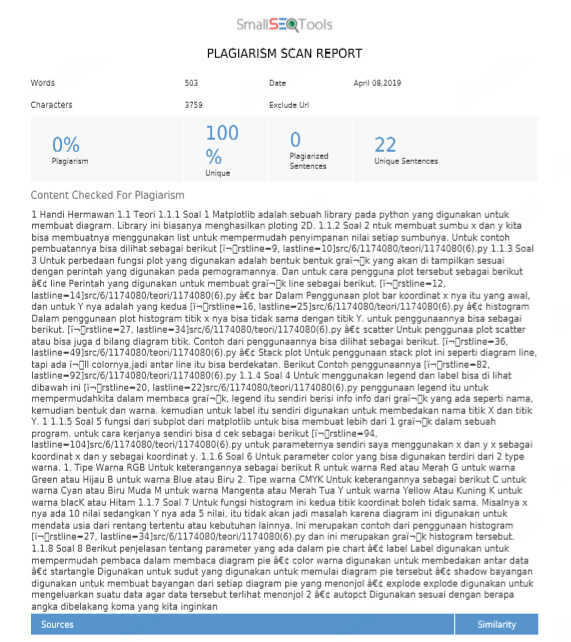
\includegraphics[width=5cm]{figures/6/1174080/teori/PLAGIARISM.PNG}
\centering
\caption{plagiarisme}
\end{figure}

%%%%%%%%%%%%%%%%%%%%%%%%%%%%%%%%%%%%%%%%%%%%%%%%%%%%%%%%%%%%%%%%%%%%%%%%%%%%%%%%%%%%%%%%%%%%%%%%%%%%%%%%%%%%%%%%%%%%


